% coding:utf-8

%FOSAET, a LaTeX-Code for a electrical summary of basic electronics
%Copyright (C) 2013, Daniel Winz, Ervin Mazlagic

%This program is free software; you can redistribute it and/or
%modify it under the terms of the GNU General Public License
%as published by the Free Software Foundation; either version 2
%of the License, or (at your option) any later version.

%This program is distributed in the hope that it will be useful,
%but WITHOUT ANY WARRANTY; without even the implied warranty of
%MERCHANTABILITY or FITNESS FOR A PARTICULAR PURPOSE.  See the
%GNU General Public License for more details.
%----------------------------------------

\subsection{Differenzierer}
\begin{figure}[h!]
	\centering
	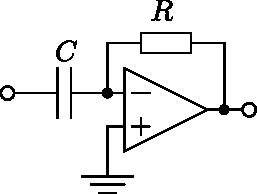
\includegraphics[scale=\schscale]{../fig/op_diff.pdf}
	\caption{Differenzierer}
	\label{sch:op-diff}
\end{figure}
\[ U_a = - R \cdot C \cdot \frac{d U_e(t)}{dt} \]
\[ X_e = \frac{1}{j \cdot \omega \cdot f \cdot C} \]
\[ R_a = 0 \]